%\RequirePackage[l2tabu, orthodox]{nag}
\documentclass[12pt]{beamer}
\graphicspath{{Imagenes/}{../Imagenes/}}
\usepackage[utf8]{inputenc}
\usepackage[spanish]{babel}
\usepackage[autostyle,spanish=mexican]{csquotes}
\usepackage{hyperref}
\hypersetup{
  colorlinks=true,
  linkcolor=blue,          % color of internal links (change box color with linkbordercolor)
  citecolor=green,        % color of links to bibliography
  filecolor=magenta,      % color of file links
  urlcolor=cyan,           % color of external links
  linkbordercolor={0 0 1}
}
\usepackage{amsmath}
\usepackage{amsthm}
\usepackage{multicol}
\usepackage{graphicx}
\usepackage{physics}
\usepackage{tabulary}
\usepackage{booktabs}
\usepackage[outdir=./]{epstopdf}
%\usepackage{epstopdf}
\usepackage{media9}
\usepackage{multimedia}
\usepackage[binary-units=true]{siunitx}
\usepackage{standalone}
\usepackage{longtable}
\usepackage{bigints}
\usepackage[font=footnotesize,textfont=it]{caption}
%\usepackage{enumitem}
\usepackage{tikz}
\usetikzlibrary{mindmap}
\usepackage[siunitx]{circuitikz}
\usetikzlibrary{arrows, patterns, shapes, decorations.markings, decorations.pathmorphing}
\usetikzlibrary{matrix,positioning}
\tikzstyle{every picture}+=[remember picture,baseline]
\usepackage{color}
\usepackage{alltt}
\usepackage{verbatim}
\usepackage{colortbl}
\usepackage{fancyvrb}
\usepackage[os=win]{menukeys}
\usepackage{pifont}
\usepackage[sfdefault]{roboto}  %% Option 'sfdefault' only if the base font of the document is to be sans serif
%\usepackage[T1]{fontenc}
\setcounter{secnumdepth}{3}
\setcounter{tocdepth}{3}
\DeclareGraphicsExtensions{.pdf,.png,.jpg}
\renewcommand {\arraystretch}{1.5}
\definecolor{ao}{rgb}{0.0, 0.5, 0.0}
\definecolor{bisque}{rgb}{1.0, 0.89, 0.77}
\definecolor{amber}{rgb}{1.0, 0.75, 0.0}
\definecolor{armygreen}{rgb}{0.29, 0.33, 0.13}
\definecolor{alizarin}{rgb}{0.82, 0.1, 0.26}
\definecolor{cadetblue}{rgb}{0.37, 0.62, 0.63}
\newcommand*{\TitleParbox}[1]{\parbox[c]{6cm}{\raggedright #1}}%
\newcommand{\python}{\texttt{python}}
\newcommand{\textoazul}[1]{\textcolor{blue}{#1}}
\newcommand{\azulfuerte}[1]{\textcolor{blue}{\textbf{#1}}}
\newcommand{\funcionazul}[1]{\textcolor{blue}{\textbf{\texttt{#1}}}}
%\normalfont
\usepackage{ccfonts}% http://ctan.org/pkg/{ccfonts}
\usepackage[T1]{fontenc}% http://ctan.or/pkg/fontenc
\renewcommand{\rmdefault}{cmr}% cmr = Computer Modern Roman
\usefonttheme[onlymath]{serif}
\linespread{1.3}
\newcounter{saveenumi}
\newcommand{\seti}{\setcounter{saveenumi}{\value{enumi}}}
\newcommand{\conti}{\setcounter{enumi}{\value{saveenumi}}}
\newcommand{\tikzmark}[1]{\tikz[remember picture] \node[coordinate] (#1) {#1};}

\usepackage{scalerel}[2016-12-29]
\def\stretchint#1{\vcenter{\hbox{\stretchto[440]{\displaystyle\int}{#1}}}}
\def\scaleint#1{\vcenter{\hbox{\scaleto[3ex]{\displaystyle\int}{#1}}}}
\def\bs{\mkern-12mu}

\newtheorem{teo}{}[section]
\usepackage{blkarray}

%reduce el tamaño de letra de la etiqueta equations
\makeatletter
\def\maketag@@@#1{\hbox{\m@th\normalfont\small#1}}
\makeatother

%se usa para la x en itemize
\newcommand{\xmark}{\text{\ding{55}}}

%\AtBeginDocument{\setlength{\tymin}{1em}}


\definecolor{myblue}{rgb}{.8, .8, 1}

\usepackage{amsmath}
\usepackage{empheq}

\newlength\mytemplen
\newsavebox\mytempbox

\makeatletter
\newcommand\mybluebox{%
    \@ifnextchar[%]
       {\@mybluebox}%
       {\@mybluebox[0pt]}}

\def\@mybluebox[#1]{%
    \@ifnextchar[%]
       {\@@mybluebox[#1]}%
       {\@@mybluebox[#1][0pt]}}

\def\@@mybluebox[#1][#2]#3{
    \sbox\mytempbox{#3}%
    \mytemplen\ht\mytempbox
    \advance\mytemplen #1\relax
    \ht\mytempbox\mytemplen
    \mytemplen\dp\mytempbox
    \advance\mytemplen #2\relax
    \dp\mytempbox\mytemplen
    \colorbox{myblue}{\hspace{1em}\usebox{\mytempbox}\hspace{1em}}}

\makeatother



\usepackage{courier}
\usepackage{listingsutf8}
\usepackage{listings}
\usepackage{xcolor}
\usepackage{textcomp}
\usepackage{color}
\definecolor{deepblue}{rgb}{0,0,0.5}
\definecolor{brown}{rgb}{0.59, 0.29, 0.0}
\definecolor{OliveGreen}{rgb}{0,0.25,0}
% \usepackage{minted}

\DeclareCaptionFont{white}{\color{white}}
\DeclareCaptionFormat{listing}{\colorbox{gray}{\parbox{0.98\textwidth}{#1#2#3}}}
\captionsetup[lstlisting]{format=listing,labelfont=white,textfont=white}
\renewcommand{\lstlistingname}{Código}


\definecolor{Code}{rgb}{0,0,0}
\definecolor{Keywords}{rgb}{255,0,0}
\definecolor{Strings}{rgb}{255,0,255}
\definecolor{Comments}{rgb}{0,0,255}
\definecolor{Numbers}{rgb}{255,128,0}

\makeatletter

\newif\iffirstchar\firstchartrue
\newif\ifstartedbyadigit
\newif\ifprecededbyequalsign

\newcommand\processletter
{%
  \ifnum\lst@mode=\lst@Pmode%
    \iffirstchar%
        \global\startedbyadigitfalse%
      \fi
      \global\firstcharfalse%
    \fi
}

\newcommand\processdigit
{%
  \ifnum\lst@mode=\lst@Pmode%
      \iffirstchar%
        \global\startedbyadigittrue%
      \fi
      \global\firstcharfalse%
  \fi
}

\lst@AddToHook{OutputOther}%
{%
  \lst@IfLastOtherOneOf{=}
    {\global\precededbyequalsigntrue}
    {}%
}

\lst@AddToHook{Output}%
{%
  \ifprecededbyequalsign%
      \ifstartedbyadigit%
        \def\lst@thestyle{\color{orange}}%
      \fi
    \fi
  \global\firstchartrue%
  \global\startedbyadigitfalse%
  \global\precededbyequalsignfalse%
}

\lstset{ 
language=Python,                % choose the language of the code
basicstyle=\footnotesize\ttfamily,       % the size of the fonts that are used for the code
numbers=left,                   % where to put the line-numbers
numberstyle=\scriptsize,      % the size of the fonts that are used for the line-numbers
stepnumber=1,                   % the step between two line-numbers. If it is 1 each line will be numbered
numbersep=5pt,                  % how far the line-numbers are from the code
backgroundcolor=\color{white},  % choose the background color. You must add \usepackage{color}
showspaces=false,               % show spaces adding particular underscores
showstringspaces=false,         % underline spaces within strings
showtabs=false,                 % show tabs within strings adding particular underscores
frame=single,   		% adds a frame around the code
tabsize=2,  		% sets default tabsize to 2 spaces
captionpos=t,   		% sets the caption-position to bottom
breaklines=true,    	% sets automatic line breaking
breakatwhitespace=false,    % sets if automatic breaks should only happen at whitespace
escapeinside={| |},  % if you want to add a comment within your code
stringstyle =\color{OliveGreen},
otherkeywords={as, np.array, np.concatenate, np.linspace, linspace, interpolate.interp1d, kind, plt.plot, .copy, np.arange, np.cos, np.pi, lw, ls, label, splrep, splev, plt.legend, loc, plt.title, plt.ylim, plt.show, sign, math.ceil, math.log, np.sqrt, np.exp, np.zeros, plt.xlabel, plt.ylabel, plt.xlim, np.identity, random, np.dot, np.outer, np.diagonal },             % Add keywords here
keywordstyle = \color{blue},
commentstyle = \color{darkcerulean},
identifierstyle = \color{black},
literate=%
         {á}{{\'a}}1
         {é}{{\'e}}1
         {í}{{\'i}}1
         {ó}{{\'o}}1
         {ú}{{\'u}}1
%
%keywordstyle=\ttb\color{deepblue}
%fancyvrb = true,
}

\lstdefinestyle{FormattedNumber}{%
    literate={0}{{\textcolor{red}{0}}}{1}%
             {1}{{\textcolor{red}{1}}}{1}%
             {2}{{\textcolor{red}{2}}}{1}%
             {3}{{\textcolor{red}{3}}}{1}%
             {4}{{\textcolor{red}{4}}}{1}%
             {5}{{\textcolor{red}{5}}}{1}%
             {6}{{\textcolor{red}{6}}}{1}%
             {7}{{\textcolor{red}{7}}}{1}%
             {8}{{\textcolor{red}{8}}}{1}%
             {9}{{\textcolor{red}{9}}}{1}%
             {.0}{{\textcolor{red}{.0}}}{2}% Following is to ensure that only periods
             {.1}{{\textcolor{red}{.1}}}{2}% followed by a digit are changed.
             {.2}{{\textcolor{red}{.2}}}{2}%
             {.3}{{\textcolor{red}{.3}}}{2}%
             {.4}{{\textcolor{red}{.4}}}{2}%
             {.5}{{\textcolor{red}{.5}}}{2}%
             {.6}{{\textcolor{red}{.6}}}{2}%
             {.7}{{\textcolor{red}{.7}}}{2}%
             {.8}{{\textcolor{red}{.8}}}{2}%
             {.9}{{\textcolor{red}{.9}}}{2}%
             {\ }{{ }}{1}% handle the space
         ,%
          %mathescape=true
          escapeinside={__}
          }



%Se usa la plantilla Warsaw modificada con spruce
\mode<presentation>
{
  \usetheme{Warsaw}
  \setbeamertemplate{headline}{}
  \useoutertheme{default}
  \usecolortheme{seahorse}
  \setbeamercovered{invisible}
}
% \AtBeginSection[]
% {
% \begin{frame}<beamer>{Contenido}
% \normalfont\mdseries
% \tableofcontents[currentsection]
% \end{frame}
%}
\makeatletter
\setbeamertemplate{footline}
{
  \leavevmode%
  \hbox{%
  \begin{beamercolorbox}[wd=.333333\paperwidth,ht=2.25ex,dp=1ex,center]{author in head/foot}%
    \usebeamerfont{author in head/foot} \textcolor{purple}{\insertsection}
  \end{beamercolorbox}}%
  \begin{beamercolorbox}[wd=.333333\paperwidth,ht=2.25ex,dp=1ex,center]{title in head/foot}%
    \usebeamerfont{title in head/foot}\insertsubsection
  \end{beamercolorbox}%
  \begin{beamercolorbox}[wd=.333333\paperwidth,ht=2.25ex,dp=1ex,right]{date in head/foot}%
    \usebeamerfont{date in head/foot}\insertshortdate{}\hspace*{2em}
    \insertframenumber{} / \inserttotalframenumber\hspace*{2ex} 
  \end{beamercolorbox}}%
  \vskip0pt%
\makeatother
\normalfont
\usepackage{ccfonts}% http://ctan.org/pkg/{ccfonts}
\usepackage[T1]{fontenc}% http://ctan.or/pkg/fontenc
\renewcommand{\rmdefault}{cmr}% cmr = Computer Modern Roman
\linespread{1.3}
\title{Métodos de Monte Carlo - 2}
\subtitle{Curso de Física Computacional}
\author[]{M. en C. Gustavo Contreras Mayén}
\setbeamercolor{background canvas}{bg=white} %white = default
\setbeamertemplate{caption}[numbered]
\beamertemplatenavigationsymbolsempty
\begin{document}
\newcommand{\localtextbulletone}{\textcolor{gray}{\raisebox{.45ex}{\rule{.6ex}{.6ex}}}}
\maketitle
\fontsize{14}{14}\selectfont
\spanishdecimal{.}
\begin{frame}{Contenido}
\tableofcontents[pausesections]
\end{frame}
\section{Métodos Monte Carlo}
\subsection{Integración Monte Carlo}
\begin{frame}
\frametitle{Integración Monte Carlo}
Una de las primeras aplicaciones con el uso de números aleatorios ha sido el cálculo numérico de integrales, es decir, un problema no aleatorio (determinista).
\\
\bigskip
Veamos un primer método para calcular
\[ \int_{a}^{b} f(x) \; d x \]
\end{frame}
\begin{frame}
\frametitle{Integración estándar Monte Carlo}
Sea $x_{1}, x_{2}, \ldots, x_{n}$ la secuencia de números aleatorios uniformemente distribuidos entre $a$ y $b$.
\\
\bigskip
Entonces
\begin{equation}
 (b - a) \; \dfrac{1}{n} \; \sum_{i=1}^{n} f(x_{i})
\label{eq:ecuacion_08_07}
\end{equation}
\end{frame}
\begin{frame}
\frametitle{Aproximación a la integral}
Es una aproximación a la integral 
\[ \int_{a}^{b} f(x) dx \]
Este método se denomina generalmente \emph{integración de Monte Carlo}.
\end{frame}
\begin{frame}
\frametitle{Aproximación a la integral}
Es fácil de interpretar la ec. (\ref{eq:ecuacion_08_07}): Un resultado bien conocido del cálculo es que la integral de una función $f$ sobre $[a, b]$ es igual al valor medio de $f$ sobre $[a, b]$ multiplicado por la longitud del intervalo, $(b - a)$.
\end{frame}
\begin{frame}
\frametitle{Aproximación a la integral}
Si aproximamos el valor medio de $f(x)$ por la media de $n$ evaluaciones de la función distribuidas al azar $f(x_{i})$, obtenemos el método de integración.
\end{frame}
\begin{frame}[plain, fragile]
\frametitle{Estimado la integral con python}
Podemos implementar la ec. (\ref{eq:ecuacion_08_07}) en una pequeña función de \python:
\begin{lstlisting}[caption=Función para aproximar la integral, style=FormattedNumber, basicstyle=\linespread{1.1}\ttfamily=\small, columns=fullflexible]
import random

def MCint(f, a, b, n):
    s = 0
    for i in range(n):
        x = random.uniform(a, b)
        s += f(x)
        
    I = (float(b-a)/n) * s
    return I
\end{lstlisting}
\end{frame}
\begin{frame}[fragile]
\frametitle{Versión más rápida del código}
Normalmente se necesita un valor de $n$ grande para obtener buenos resultados con este método, por lo que una versión vectorizada más rápida de la función anterior es útil:
\end{frame}
\begin{frame}[plain, fragile]
\frametitle{Versión más rápida del código}
\begin{lstlisting}[caption=Función vectorizada para la aproximación de la integral, style=FormattedNumber, basicstyle=\linespread{1.1}\ttfamily=\small, columns=fullflexible]
import random
from numpy import *

def MCintvec(f, a, b, n):
    x = random.uniform(a, b, n)
    s = sum(f(x))
    I = (float(b-a)/n) * s
    return I
\end{lstlisting}
\end{frame}
\begin{frame}
\frametitle{Ejemplo}
Vamos a probar el método de integración de Monte Carlo en una función simple, sea $f(x) = 2 + 3 \: x$, y calculemos la integral en $[1, 2]$.
\\
\bigskip
La mayoría de los otros métodos de integración numérica resolverán exactamente esa función lineal, independientemente del número de evaluaciones de la función.
\end{frame}
\begin{frame}
\frametitle{Ejemplo}
Este no es el caso de la integración de Monte Carlo. 
\\
\bigskip
Sería interesante ver cómo la calidad de la aproximación de Monte Carlo se incrementa, conforme crece el valor de $n$.
\end{frame}
\begin{frame}
\frametitle{Ejemplo}
Para graficar la evolución de la aproximación con la integral, debemos almacenar los valores intermedios $I$, por lo que debemos de modificar el código:
\end{frame}
\begin{frame}[plain, fragile]
\begin{lstlisting}[caption=Código para el ejercicio, style=FormattedNumber, basicstyle=\linespread{1.1}\ttfamily=\small, columns=fullflexible]
def MCint_2_(f, a, b, n):
    # se guardan las aproximaciones intermedias de la integral en el arreglo I,
    # donde I[k-_1_] es k veces la funcion evaluada
    s = 0

    I = np.zeros(n)

    for k in range(1, n+1):
        x = random.uniform(a, b)
        s += f(x)
        I[k-_1_] = (float(b-a)/k) * s
    return I
\end{lstlisting}
\end{frame}
\begin{frame}
\frametitle{Consideraciones para la solución}
Toma en cuenta que hacemos que $k$ vaya de $1$ a $n$ mientras que los índices en $I$, como de costumbre, van de $0$ a $n-1$.
\end{frame}
\begin{frame}
\frametitle{Consideraciones para la solución}
Dado que $n$ puede ser muy grande, el arreglo $I$ puede consumir más memoria de lo que tenemos disponible en la computadora.
\\
\bigskip
Por lo tanto, decidimos almacenar sólo cada $N$ valores de la aproximación. 
\end{frame}
\begin{frame}[plain, fragile]
\frametitle{Consideraciones para la solución}
El determinar si un valor debe ser almacenado o no puede ser calculado por la función \texttt{mod}:
\begin{lstlisting}[caption=Almacenamiento de valores, style=FormattedNumber, basicstyle=\linespread{1.1}\ttfamily=\small, columns=fullflexible]
for k in range(1, n+_1_):
    if k % N == 0:
    	#se guarda
\end{lstlisting}
Es decir, cada vez que $k$ se divide $N$ sin ningún residuo, almacenamos el valor.
\end{frame}
\begin{frame}[plain, allowframebreaks, fragile]
\frametitle{Código completo}
La función completa sería:
\begin{lstlisting}[caption=Código completo para el ejercicio, style=FormattedNumber, basicstyle=\linespread{1.1}\ttfamily=\small, columns=fullflexible]
def MCint_3_(f, a, b, n, N=100):
    s = 0
    Ivalores = []
    kvalores = []
    
    for k in range(1, n+1):
        x = random.uniform(a, b)
        s += f(x)
        if k % N == 0:
            I = (float(b-a)/k) * s
            Ivalores.append(I)
            kvalores.append(k)
    
    return k_valores, I_valores
\end{lstlisting}
\end{frame}
\begin{frame}[plain, fragile]
\frametitle{Estimación del error}
Ahora podemos revisar el error que se genera al usar la función:
\begin{lstlisting}[caption=Estimación del error del procedimiento, style=FormattedNumber, basicstyle=\linespread{1.1}\ttfamily=\small, columns=fullflexible]
def f_1_(x):
    return 2 + 3*x


k, I = MCint_3_(f_1_, 1, 2, 1000000, N=10000)

error = 6.5 - np.array(I)
\end{lstlisting}
\end{frame}
\begin{frame}[fragile]
\frametitle{Gráfica del error vs $N$}
\begin{figure}
	\centering
	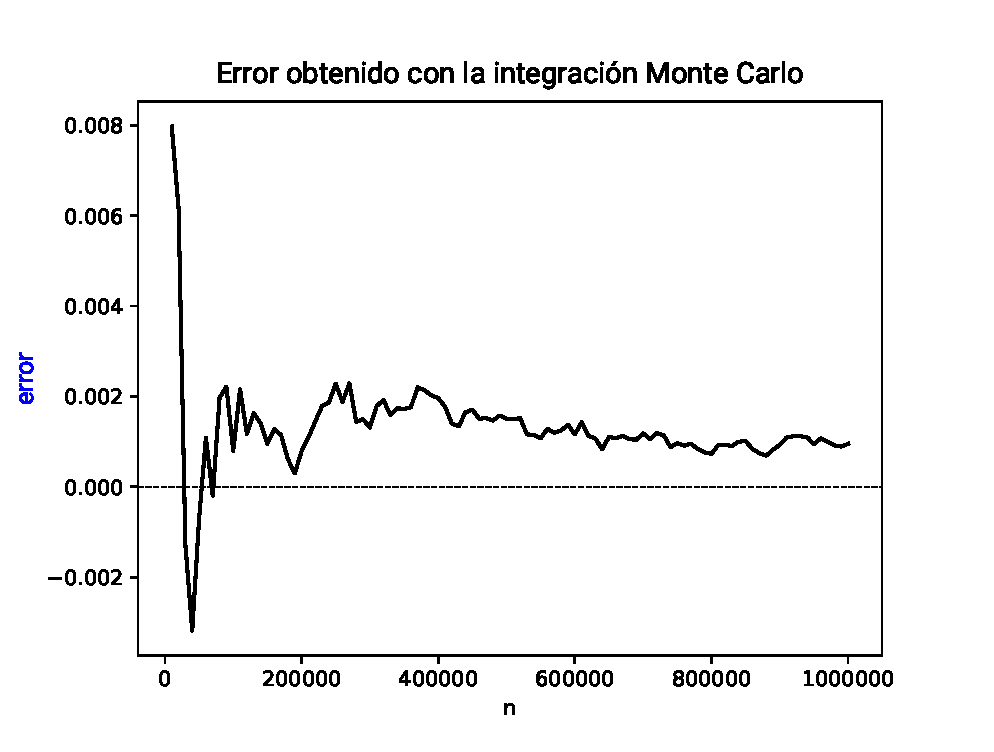
\includegraphics[scale=0.55]{Imagenes/integracionMC01_2017.eps}
	\caption{Convergencia de la integración de Monte Carlo para $f(x)$}
\end{figure}
\end{frame}
\begin{frame}
\frametitle{Velocidad de convergencia}
Para funciones de una variable, el método (\ref{eq:ecuacion_08_07}) requiere de muchos puntos y es ineficiente comparado con otras reglas de integración.
\\
\bigskip
La mayoría de las reglas de integración tienen un error que se reduce mientras se incrementa $n$, normalmente de la manera $n^{-r}$ para un $r>0$.
\end{frame}
\begin{frame}
\frametitle{Velocidad de convergencia}
Para la regla del trapecio, $r = 2$, mientras que para la integración de Monte Carlo $r = 1/2$
\\
\bigskip
Esto significa que este método converge muy lentamente en comparación con la regla del trapecio.
\end{frame}
\subsection{Integración en varias variables}
\begin{frame}
\frametitle{Integración en varias variables}
Sin embargo, para funciones de varias variables, la integración de Monte Carlo en espacios de dimensiones mayores supera completamente a métodos como la regla del trapecio y la regla de Simpson.
\end{frame}
\begin{frame}
\frametitle{Mejoras para el cálculo de la integral}
Existen diferentes maneras de mejorar el rendimiento de la ec. (\ref{eq:ecuacion_08_07}), básicamente por ser \enquote{aplicados} al momento de graficar los números aleatorios, conocidas como técnicas de reducción de la varianza.
\end{frame}
\subsection{Calculando áreas con puntos aleatorios}
\begin{frame}
\frametitle{Calculando áreas con puntos aleatorios}
Pensemos en alguna región geométrica $G$ en el plano y una caja circundante $B$ con geometría $[x_{L}, x_{H}] \times [y_{L}, y_{H}]$.
\\
\bigskip
Una forma de calcular el área de $G$ es dibujar $N$ puntos aleatorios dentro de $B$ y contar cuántos de ellos $M$, están dentro de $G$.
\end{frame}
\begin{frame}
\frametitle{Puntos dentro de la región}
El área de $G$ es entonces la fracción $M/N$ (fracción de $G$ en el área de $B$) veces el área de $B$, $(x_{H} - x_{L})(y_{H} - y_{L})$.
\end{frame}
\begin{frame}
\frametitle{Puntos dentro de la región}
De forma diferente, este método es una especie de juego de dardos en el que se cuentan los que caen dentro de $G$, si cada lanzamiento llega de manera uniforme dentro de $B$.
\end{frame}
\begin{frame}
\frametitle{Calculando una integral}
Veamos cómo será la expresión para calcular la integral
\[ \int_{a}^{b} f(x) \: dx \]
Como nota relevante, consideremos que esta integral es el área debajo de la curva $y = f(x)$ y sobre el eje $x$, entre $x = a$ y $x = b$.
\end{frame}
\begin{frame}
\frametitle{Calculando una integral}
Introducimos un rectángulo $B$, tal que
\[ B = \{ (x, y) \vert a \leq x \leq b, \hspace{0.3cm} 0 \leq y \leq m \} \]
donde $m \leq \max_{x \in [a, b]} \; f(x)$
\end{frame}
\begin{frame}
\frametitle{Calculando una integral}
El algoritmo para calcular el área bajo la curva se basa en dibujar $N$ puntos aleatorios dentro de $B$ y contar cuántos de ellos, $M$, están por encima del eje $x-y$  y cuántos por debajo de la curva $y=f(x)$
\end{frame}
\begin{frame}
\frametitle{Método del dardo}
\begin{figure}
	\centering
	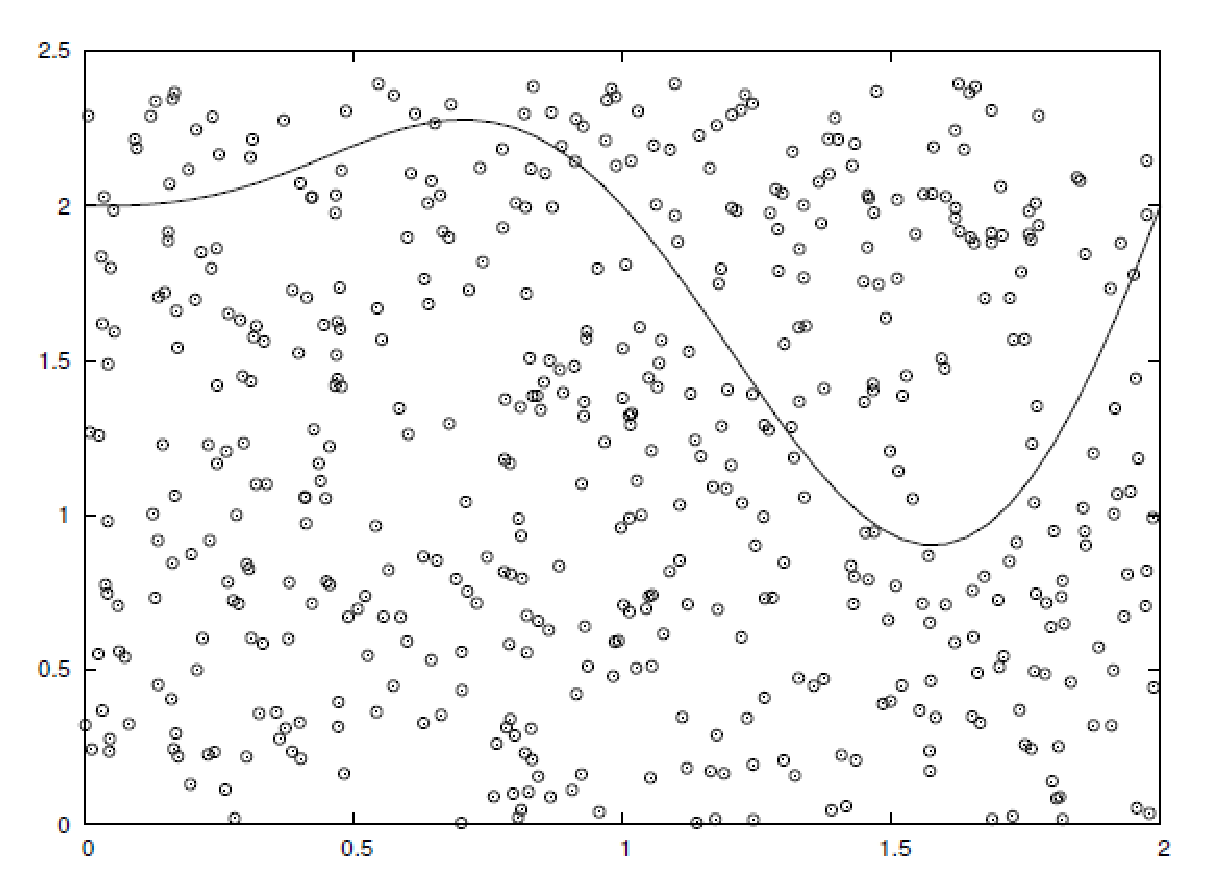
\includegraphics[scale=0.4]{Imagenes/integracionCaja.eps}
	\caption{\tiny{Cuando $M$ de $N$ puntos aleatorios en el rectángulo $[0, 2] \times [0, 2.4]$ se encuentran bajo la curva, el área bajo la curva se estima como la fracción $M / N$ del área del rectángulo.}}
\end{figure}
\end{frame}
\begin{frame}
\frametitle{Valor de la integral}
El área o el valor de la integral se estima por la expresión
\[ \dfrac{M}{N} \: m \: (b - a) \]
\\
\bigskip
El código sería
\end{frame}
\begin{frame}[plain, fragile]
\frametitle{Código para la integral}
\begin{lstlisting}[caption=Código para el método del dardo, style=FormattedNumber, basicstyle=\linespread{1.1}\ttfamily=\small, columns=fullflexible]
def MCint-area(f, a, b, n, m):
    porDebajo = 0 
    for i in range(n):
        x = random.uniform(a, b)
        y = random.uniform(0, m)
        if y <= f(x):
            porDebajo += 1
    area = porDebajo/float(n) * m * (b - a)
    
    return area
\end{lstlisting}
\end{frame}
\begin{frame}[fragile]
Toma en cuenta que este método opera con el doble de números aleatorios que el método anterior.
\\
\bigskip
Una implementación vectorizada del código es
\begin{lstlisting}[caption=Método del dardo en modo vectorizado, style=FormattedNumber, basicstyle=\linespread{1.1}\ttfamily=\small, columns=fullflexible]
def MCint-area-vec(f, a, b, n, m):
    x = random.uniform(a, b, n)
    y = random.uniform(0, m, n)
    porDebajo = np.sum(y < f(x))
    area = porDebajo/float(n) * m * (b - a)
    
    return area
\end{lstlisting}
\end{frame}
\begin{frame}
Podemos ejecutar el código para un conjunto de 2 millones de números al azar, la versión de bucle sencillo no es tan lenta.
\\
\bigskip
Sin embargo, si necesita que la integración se repita muchas veces dentro de otro cálculo, puede ser importante la eficacia superior de la versión vectorizada.
\end{frame}
\begin{frame}[plain, allowframebreaks, fragile]
\frametitle{Función completa}
\begin{lstlisting}[caption=Función para el método del dardo, style=FormattedNumber, basicstyle=\linespread{1.1}\ttfamily=\small, columns=fullflexible]
def MCint_3_area(f, a, b, n, m, N=1000):
    Ivalores = []
    kvalores = []
    porDebajo = 0
    for k in range(1, n+1):
        x = random.uniform(a, b)
        y = random.uniform(0, m)
        if y <= f(x):
            porDebajo += 1
        area = porDebajo/float(k) * m * (b-a)
        if k % N == 0:
            I = area
            Ivalores.append(I)
            kvalores.append(2 * k)
    return kvalores, Ivalores
\end{lstlisting}
\end{frame}
\begin{frame}
\frametitle{Implementación del código}
Al contar con los elementos necesarios, podemos implementar el código completo para estimar el valor de la integral a partir de generar puntos aleatorios.
\\
\bigskip
Haremos una estimación del tiempo que tarda en resolverse el problema usando el bucle y la versión vectorizada.
\end{frame}
\begin{frame}
\frametitle{La librería \funcionazul{time}}
La librería \funcionazul{time} proporciona un conjunto de funciones para registrar el tiempo en el equipo de cómputo.
\\
\bigskip
Revisa la documentación de la librería, ya que tiene como punto particular el hecho de medir el tiempo a partir del 1 de enero de 1970, al momento actual en el equipo.
\end{frame}
\begin{frame}
\frametitle{Para medir un intervalo}
Para el ejercicio que haremos, se requiere medir un intervalo de tiempo entre dos eventos, por lo que no es necesario hacer alguna conversión de tiempo.
\\
\bigskip
La función \funcionazul{time.clock()} hará el registro del tiempo en el equipo, para el intervalo, basta con que hagamos un segundo registro y tomar la diferencia entre éstos.
\end{frame}
\begin{frame}[plain, allowframebreaks, fragile]
\begin{lstlisting}[caption=Implementación del código, style=FormattedNumber, basicstyle=\linespread{1.1}\ttfamily=\small, columns=fullflexible]
def f_1_(x):
    return 2 + 3 * x

a = 1; b = 2; n = 1000000; N = 10000; fmax = f_1_(b)

t_0_ = time.clock()

print (MCintarea(f_1_, a, b, n, fmax))

t_1_ = time.clock()

print (MCintareavec(f_1_, a, b, n, fmax))

t_2_ = time.clock()

print ('fraccion bucle/vectorizada:', (t_1_ - t_0_)/(t_2_ - t_1_))

k, I = MCint_3_area(f_1_, a, b, n, fmax, N)

print (I[-_1_])

error = 6.5 - np.array(I)
\end{lstlisting}
\end{frame}
\begin{frame}
\frametitle{Graficando los puntos}
A continuación se presenta una gráfica con los puntos aleatorios debajo de la función y por arriba de ésta.
\\
\bigskip
No tendrás problema para implementar el código necesario para las gráficas.
\end{frame}
\begin{frame}
\frametitle{Gráfica de la función}
\begin{figure}
	\centering
	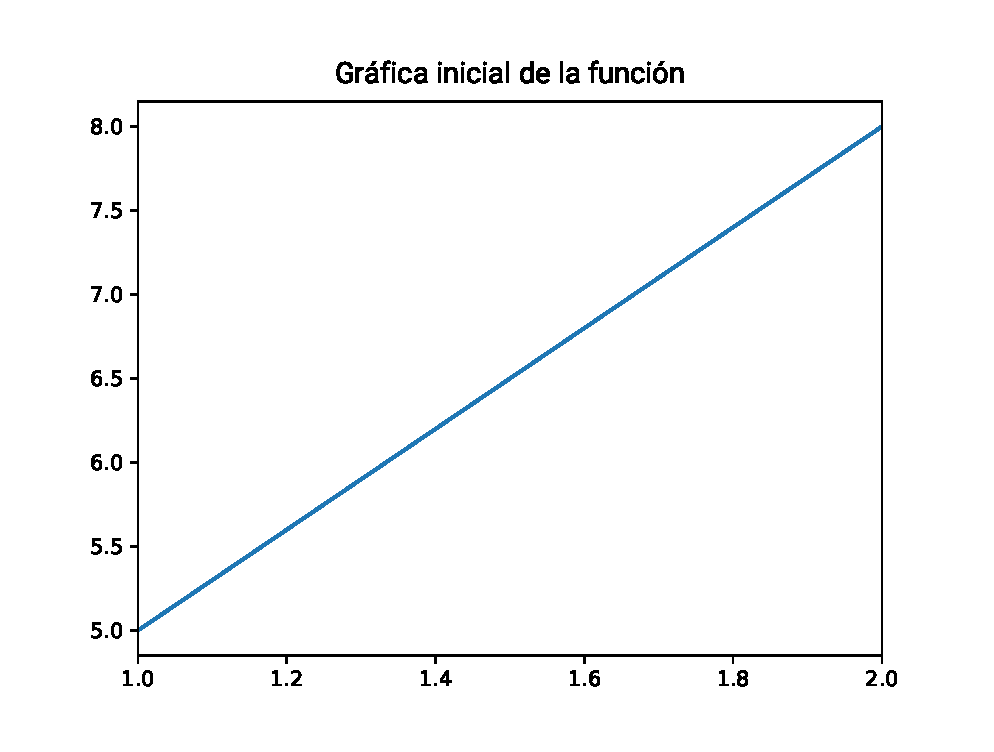
\includegraphics[scale=0.55]{Imagenes/area_puntos_01.eps}
    \caption{Función inicial.}
\end{figure}
\end{frame}
\begin{frame}
\frametitle{Gráfica al incluir puntos aleatorios}
\begin{figure}
    \centering
    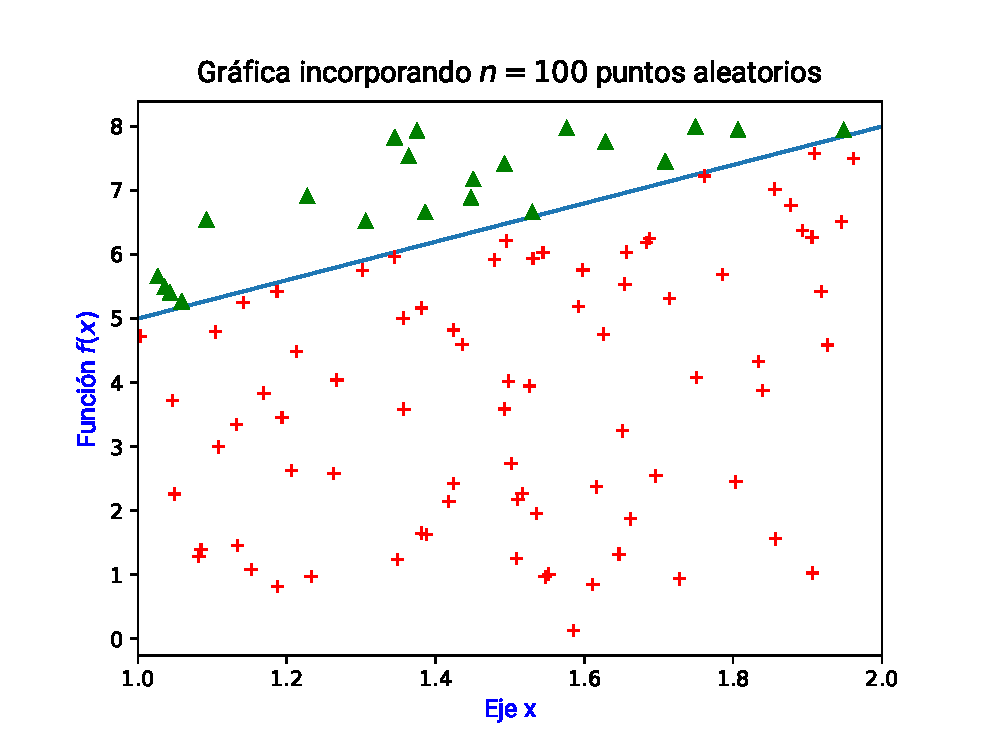
\includegraphics[scale=0.55]{Imagenes/area_puntos_02.eps}
    \caption{Puntos por arriba y por debajo de la función.}
\end{figure}
\end{frame}
\begin{frame}
\frametitle{Gráfica al incluir puntos aleatorios}
\begin{figure}
    \centering
    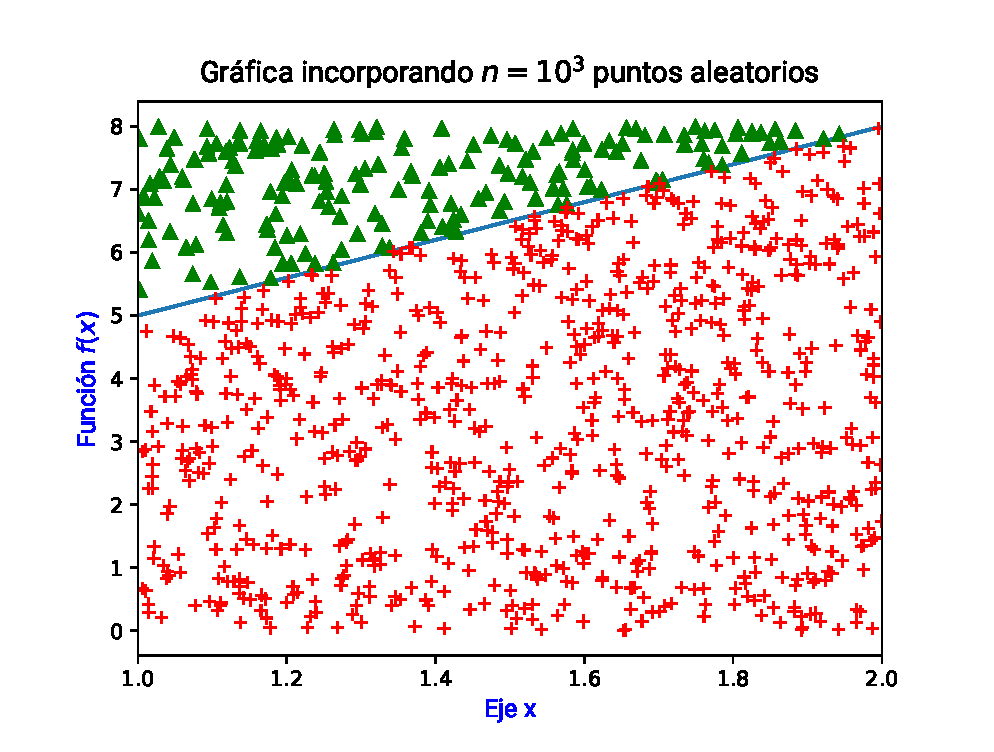
\includegraphics[scale=0.55]{Imagenes/area_puntos_03.eps}
    \caption{Se va saturando el área debajo de la curva.}
\end{figure}
\end{frame}
\begin{frame}
\frametitle{Gráfica al incluir puntos aleatorios}
\begin{figure}
    \centering
    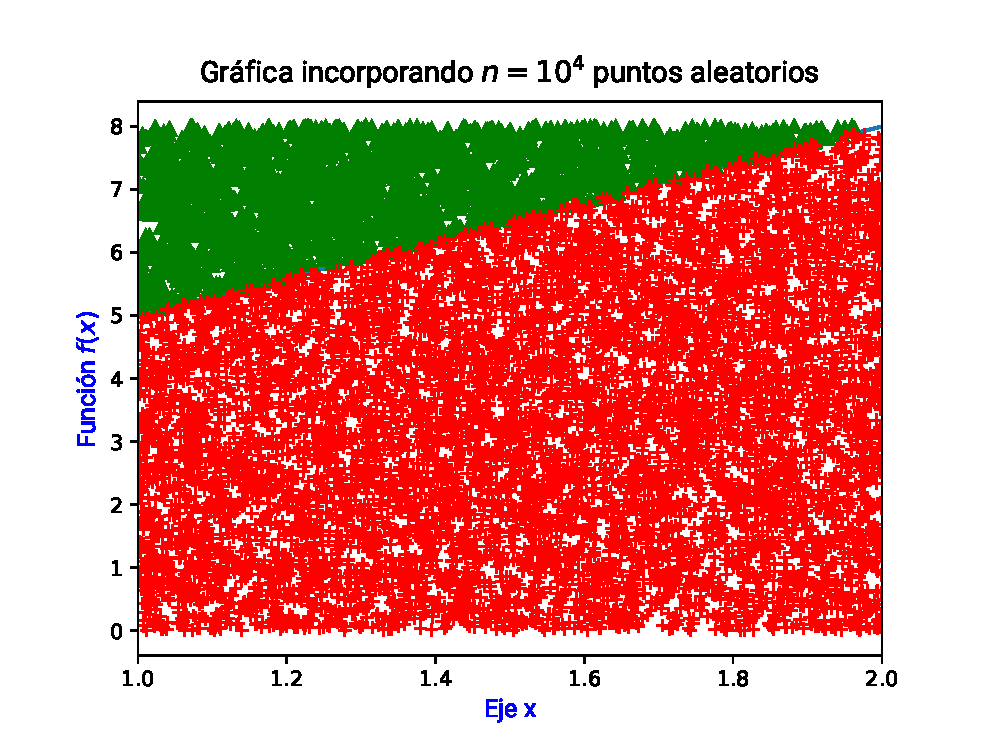
\includegraphics[scale=0.55]{Imagenes/area_puntos_04.eps}
    \caption{Casi se cubre el área debajo de la curva.}
\end{figure}
\end{frame}
\begin{frame}
\frametitle{Gráfica al incluir puntos aleatorios}
\begin{figure}
    \centering
    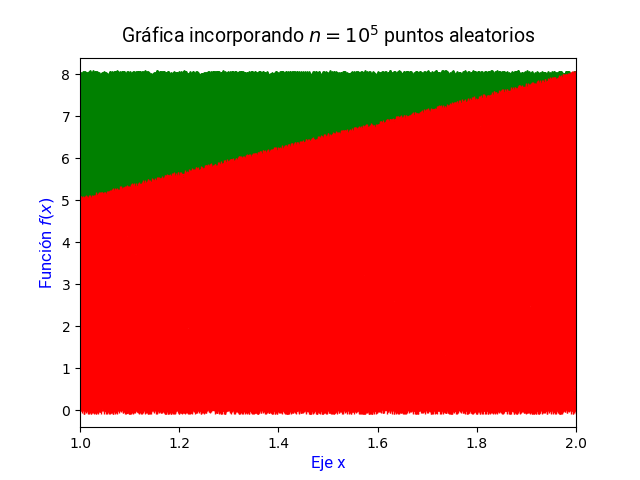
\includegraphics[scale=0.55]{Imagenes/area_puntos_05.png}
    \caption{Podríamos pensar que ya tenemos el valor de la integral.}
\end{figure}
\end{frame}
\begin{frame}
\frametitle{Gráfica al incluir puntos aleatorios}
\begin{figure}
    \centering
    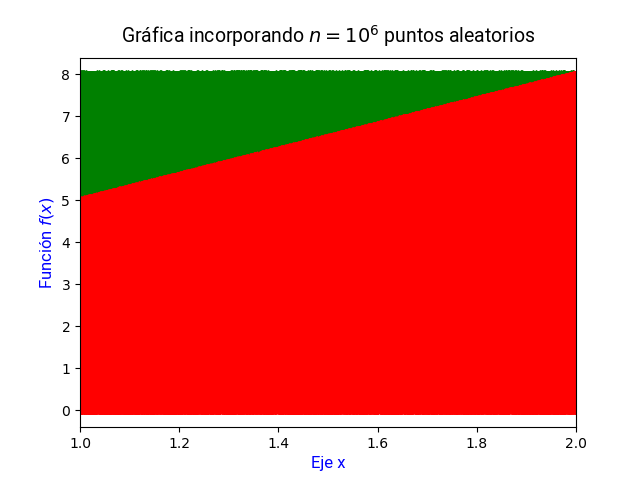
\includegraphics[scale=0.55]{Imagenes/area_puntos_06.png}
    \caption{El resultado del cálculo de la integral es exacto.}
\end{figure}
\end{frame}
\begin{frame}
\frametitle{Gráfica del error vs. número de muestras}
\begin{figure}
    \centering
    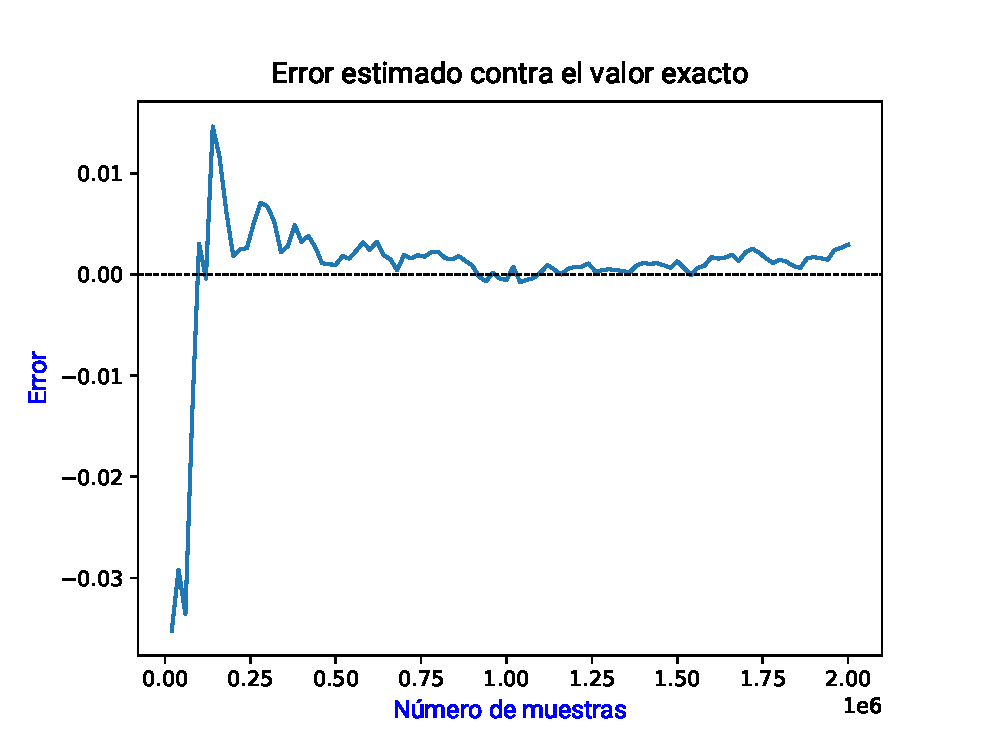
\includegraphics[scale=0.55]{Imagenes/area_puntos_07_error.eps}
    \caption{Comportamiento del error.}
\end{figure}
\end{frame}
\end{document}